% !TEX root = task-3-19-5.tex
% Editable task bank. Append new BankTask blocks at the end of the document.
\documentclass[12pt,a4paper]{article}
\usepackage{physics-textbook}
\usepackage{graphicx,needspace}
\usetikzlibrary{decorations.pathmorphing}
\newif\ifShowSolutions
\ifdefined\TutorEdition
  \ShowSolutionstrue
\else
  \ShowSolutionsfalse % Change to \ShowSolutionstrue to display solutions.
\fi
\newcounter{banktask}
\newsavebox{\BankTaskBox}
\newcommand{\BankTaskContent}[3]{%
  \noindent\textbf{\thebanktask.}\quad #2\par
  \ifShowSolutions
    \Needspace{50mm}% Keep the solution heading with its opening text or diagram.
    #3\par
    \ifdefined\TutorEdition
      \ifcsname TutorSource#1\endcsname
        \nopagebreak\smallskip{\small\csname TutorSource#1\endcsname\par}%
      \fi
    \fi
  \fi
}
\newcommand{\BankTask}[3]{%
  \refstepcounter{banktask}\par\medskip
  \sbox{\BankTaskBox}{\begin{minipage}{\linewidth}%
    \BankTaskContent{#1}{#2}{#3}\end{minipage}}%
  \ifdim\dimexpr\ht\BankTaskBox+\dp\BankTaskBox\relax>\dimexpr\textheight-20mm\relax
    \Needspace{35mm}\BankTaskContent{#1}{#2}{#3}%
  \else
    \Needspace{\dimexpr\ht\BankTaskBox+\dp\BankTaskBox\relax}%
    \noindent\usebox{\BankTaskBox}\par
  \fi
  \medskip
}
\begin{document}
\BookSubsection{3.19.5}{Взаимодействие магнита с контуром}


% Source 4E567B: https://ege.fipi.ru/bank/questions.php?search=1&proj=BA1F39653304A5B041B656915DC36B38&qid=4E567B
\BankTask{4E567B}{
В медное кольцо № 1 вносят северный полюс полосового магнита, а в пластмассовое кольцо № 2 -- южный полюс такого же магнита (см. рисунок).
\begin{enumerate}
\item В кольце № 1 индукционный ток не возникает.
\item В кольце № 2 возникает индукционный ток.
\item Кольцо № 1 притягивается к магниту.
\item Кольцо № 2 не взаимодействует с магнитом.
\item В кольце № 1 возникает ЭДС индукции.
\end{enumerate}
\begin{center}
\begin{tikzpicture}[book diagram,x=0.025cm,y=0.025cm,line join=round]
\begin{scope}
\fill[gray!35] (48,20)--(94,20)--(113,39)--(113,80)--(67,80)--(48,61)--cycle;
\draw (1,20)--(94,20)--(113,39)--(113,80)--(21,80)--(1,61)--cycle;
\draw (1,61)--(94,61)--(113,80);
\draw (94,20)--(94,61);
\draw (48,20)--(48,61)--(67,80);
\node[font=\large] at (24,40) {$S$};
\node[font=\large] at (72,40) {$N$};
\draw[-{book tip}] (38,7)--(70,7);
\fill[gray!35] (144,53) ellipse[x radius=19,y radius=51];
\fill[white] (151,53) ellipse[x radius=12,y radius=51];
\draw (144,53) ellipse[x radius=19,y radius=51];
\draw (151,53) ellipse[x radius=12,y radius=51];
\draw (146,103) .. controls (130,84) and (131,22) .. (145,3);
\node[above] at (144,112) {№ 1};
\end{scope}
\begin{scope}[xshift=6cm]
\fill[gray!35] (1,20)--(48,20)--(48,61)--(67,80)--(21,80)--(1,61)--cycle;
\draw (1,20)--(94,20)--(113,39)--(113,80)--(21,80)--(1,61)--cycle;
\draw (1,61)--(94,61)--(113,80);
\draw (94,20)--(94,61);
\draw (48,20)--(48,61)--(67,80);
\node[font=\large] at (24,40) {$N$};
\node[font=\large] at (72,40) {$S$};
\draw[-{book tip}] (38,7)--(70,7);
\fill[gray!80] (144,53) ellipse[x radius=19,y radius=51];
\fill[white] (151,53) ellipse[x radius=12,y radius=51];
\draw (144,53) ellipse[x radius=19,y radius=51];
\draw (151,53) ellipse[x radius=12,y radius=51];
\draw (146,103) .. controls (130,84) and (131,22) .. (145,3);
\node[above] at (144,112) {№ 2};
\end{scope}
\end{tikzpicture}
\end{center}
}{
\smallskip\noindent\textbf{Решение от GPT}\par
При внесении магнита поток через медное кольцо меняется, поэтому возникает ЭДС $\mathcal E=-\Delta\Phi/\Delta t$ и индукционный ток: утверждение 1 неверно, а 5 верно. Пластмасса является диэлектриком, поэтому индукционный ток в кольце № 2 не возникает: утверждение 2 неверно. По правилу Ленца медное кольцо препятствует приближению магнита и отталкивается от него, поэтому утверждение 3 неверно. Пластмассовое кольцо в рассматриваемом опыте с магнитом не взаимодействует, поэтому утверждение 4 верно. Ответ: 4, 5.
}

% Source D91D57: https://ege.fipi.ru/bank/questions.php?search=1&proj=BA1F39653304A5B041B656915DC36B38&qid=D91D57
\BankTask{D91D57}{
Медное кольцо на горизонтальном коромысле поворачивается вокруг вертикальной оси $OB$ под действием движущегося магнита (см. рисунок).

Установите соответствие между направлением движения магнита, вращением коромысла с кольцом и направлением индукционного тока в кольце (1 --- верхняя точка кольца; 2 --- ближняя к нам точка кольца; 3 --- нижняя точка кольца).

\TaskMatchingColumns[0.39\linewidth]{Направление движения магнита}{
А) движется по направлению к кольцу\par
Б) движется по направлению от кольца
}{Поворот коромысла и ток в кольце}{
1) Коромысло с кольцом поворачивается, отталкиваясь от магнита; ток идёт по направлению $3\to2\to1$.\par
2) Коромысло с кольцом поворачивается, отталкиваясь от магнита; ток идёт по направлению от $1\to2\to3$.\par
3) Коромысло с кольцом поворачивается, притягиваясь к магниту; ток идёт по направлению от $3\to2\to1$.\par
4) Коромысло с кольцом поворачивается, притягиваясь к магниту; ток идёт по направлению от $1\to2\to3$.
}

\begin{center}
\begin{tabular}{|c|c|}
\hline
А & Б \\
\hline
\phantom{0} & \phantom{0} \\
\hline
\end{tabular}
\end{center}

\begin{center}
\begin{tikzpicture}[book diagram, x=0.035cm,y=0.035cm,line cap=round,line join=round]
\filldraw[fill=gray!45,draw=black] (173,14) ellipse[x radius=35,y radius=13];
\draw (173,17)--(173,154);
\fill (173,17) circle[radius=1.5];
\node[above right] at (173,22) {$B$};
\node[above left] at (173,154) {$O$};
\draw (173,154)--(202,202)--(202,178);
\draw (146,58)--(146,108)--(173,154);
\draw (146,58)--(165,88);
\draw (118,29)--(146,72);
\draw (124,69)--(165,69);
\draw (146,69) ellipse[x radius=11,y radius=40];
\draw[line width=1.1pt] (146,109) arc[start angle=90,end angle=270,x radius=11,y radius=40];
\draw (146,29)--(146,109);
\draw (135,52)--(157,86);
\node[above left] at (146,109) {1};
\node[left] at (135,57) {2};
\node[below left] at (146,29) {3};
\draw (0,69)--(146,69);
\draw[gray] (12,77) .. controls (12,94) and (81,94) .. (81,77) .. controls (81,63) and (12,63) .. (12,77);
\draw[gray] (12,57) .. controls (12,73) and (81,73) .. (81,57) .. controls (81,43) and (12,43) .. (12,57);
\filldraw[fill=gray!65] (30,60)--(43,60)--(43,73)--(30,73)--cycle;
\filldraw[fill=gray!35] (43,60)--(59,60)--(59,73)--(43,73)--cycle;
\filldraw[fill=gray!20] (30,73)--(39,81)--(52,81)--(43,73)--cycle;
\filldraw[fill=gray!10] (43,73)--(52,81)--(67,81)--(59,73)--cycle;
\filldraw[fill=gray!45] (59,60)--(67,68)--(67,81)--(59,73)--cycle;
\node at (35,52) {$S$};
\node at (55,52) {$N$};
\filldraw[fill=white] (192,161)--(192,177) arc[start angle=180,end angle=360,x radius=10,y radius=5] --(212,161) arc[start angle=0,end angle=-180,x radius=10,y radius=5];
\draw[fill=white] (202,177) ellipse[x radius=10,y radius=5];
\draw (202,177)--(202,195);
\end{tikzpicture}
\end{center}
}{
\smallskip\noindent\textbf{Решение от GPT}\par
К кольцу обращён северный полюс магнита. По правилу Ленца при приближении магнита кольцо отталкивается; со стороны магнита у него образуется северный полюс, что соответствует току $3\to2\to1$ (вариант 1). При удалении магнита кольцо притягивается; ток меняет направление на $1\to2\to3$ (вариант 4). Ответ: А --- 1, Б --- 4.
}

% Source 2914: https://phys-ege.sdamgia.ru/problem?id=2914
\BankTask{2914}{
\begin{center}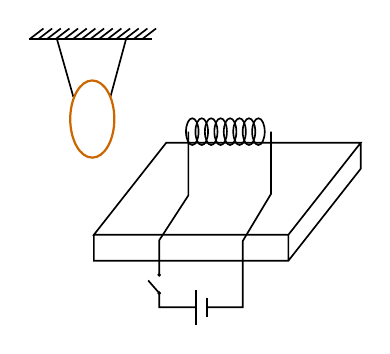
\begin{tikzpicture}[>=stealth,line width=.6pt]

\draw(-.65,2.88)--(.92,2.88);
\foreach \x in {-.63,-.52,...,.86}{\draw(\x,2.88)--++(.17,.13);}
\draw(-.29,2.88)--(-.08,2.14) (.59,2.88)--(.39,2.14);
\draw[orange!80!black,thick](.16,1.86)ellipse(.28 and .49);
\draw (.18,.39)--(2.65,.39)--(3.57,1.56)--(1.1,1.56)--cycle
 (.18,.39)--(.18,.06)--(2.65,.06)--(2.65,.39) (2.65,.06)--(3.57,1.23)--(3.57,1.56);
\draw(1.38,1.7)--(1.38,.89)--(1.01,.32)--(1.01,-.12) (2.43,1.7)--(2.43,.91)--(2.07,.31)--(2.07,-.53)--(1.62,-.53)
 (1.48,-.53)--(1.01,-.53)--(1.01,-.35);
\draw(1.01,-.35)--(.87,-.19);\fill(1.01,-.12)circle(.025) (1.01,-.35)circle(.025);
\foreach \x in {1.43,1.55,...,2.39}{\draw(\x,1.70)ellipse(.08 and .17);}
\draw(1.48,-.75)--(1.48,-.31) (1.62,-.65)--(1.62,-.41);

\end{tikzpicture}\end{center}
Замкнутое медное кольцо подвешено на длинных нитях вблизи катушки индуктивности, закрепленной на столе и подключенной к источнику постоянного тока (см. рис.). Первоначально электрическая цепь катушки разомкнута. Как будет двигаться кольцо при замыкании цепи? Ответ поясните, используя физические закономерности.
}{
\smallskip\noindent\textbf{Решение}\par
$1$.  При замыкании цепи катушки начинает изменяться поток вектора магнитной индукции через кольцо. По закону электромагнитной индукции в кольце возникает ЭДС индукции, появляется индукционный ток. В соответствии с правилом Ленца взаимодействие токов в кольце и в катушке приводит к тому, что кольцо отталкивается от катушки.
$2$.  Затем кольцо возвращается в исходное положение, так как ток в катушке достигает максимального значения, вследствие чего поток вектора магнитной индукции через кольцо становится постоянным. Индукционный ток в отсутствии ЭДС индукции затухает. Кольцо перестает отталкиваться от катушки.
$3$.  Индукционный ток в неподвижном кольце вблизи катушки с постоянным током равен нулю, магнитные свойства меди выражены слабо, поэтому, вернувшись в исходное положение равновесия, кольцо остается неподвижным.
}

\end{document}
